%07/03 - Myriam
\chapter{Dinámica molecular}
\section{Conceptos teóricos}
La dinámica molecular es la simulación informática en la que átomos y moléculas interactúan durante un periodo de tiempo y los movimientos de las distintas partículas pueden visualizarse a posteriori. No tiene en cuenta los movimientos de los electrones, considerando la energía de las moléculas en función de los movimientos de sus núcleos, siendo así ideal para macromoléculas. La mecánica clásica se basa en las leyes de Newton. Las ecuaciones de movimiento se resuelven para predecir las posiciones y velocidades de los átomos en cada paso temporal.

La aproximación de Born-Oppenheimer dice que la energía de una molécula en su estado basal puede considerarse como una función de las coordenadas de los núcleos atómicos. Los campos de fuerza permiten calcular las fuerzas de los átomos. Algunos ejemplos de campos de fuerza que se usan son GAFF, AMBER y CHARMM.

Los pasos de una dinámica molecular son:
\begin{enumerate}
\item Preparación del sistema: se hace a partir de fuentes experimental o teóricas. La parametrización incluye cargas formales, adaptación del ligando y la proteína, etc. A continuación el sistema se mete en una caja de agua. La idea es que se simula un sistema con condiciones fisiológicas como si fuera un experimento real.
\item Minimización: consiste en minimizar el complejo y la caja de agua. Hace referencia a que el sistema esté estable y en equilibrio.
\item Calentamiento: se pueden tener varias etapas de calentamiento con un máximo de 300 K. Si hay varias, se pueden hacer de forma progresiva. En los artículos que utilicen dinámica molecular, suelen indicar las condiciones (temperatura, presión, duración de la dinámica, etc.)
\item Equilibrado: se trabaja en condiciones normales con presión de 1 atmósfera generalmente, pero hay que ajustarlo siempre.
\item Producción: es la etapa de dinámica molecular, el paso importante. Si todo ha ido bien en los pasos anteriores, no debería haber problemas, mientras que si algo falla, se deben añadir restricciones u otros parámetros. Aquí es donde realmente se establece la duración de la dinámica. Cuanto mayor duración, más espacio explorable tiene la molécula y mayor tiempo de cálculo se necesita. La producción produce la trayectoria.
\end{enumerate}

La dinámica molecular se utiliza para:
\begin{itemize}
\item Se estudian procesos como la apertura y cierre de canales iónicos, cambios en la estructura de proteínas reguladoras...
\item Estudio de la estabilidad de los complejos
\item Se analizan las posibles rutas de plegamiento y se identifican estados intermedios metaestables. 
\item Estudio de la cinética del crecimiento de cristales en soluciones y su relación con la estabilidad de los fármacos.
\item La interacción de las moléculas con la bicapa lipídica se estudia para comprender su permeabilidad y absorción en los sistemas biológicos.
\end{itemize}

Después de la dinámica molecular se suelen hacer algunos \textbf{análisis de estabilidad}:
\begin{itemize}
\item \textbf{RMSD}: Evaluación de los cambios conformacionales de una molécula o complejo a lo largo del tiempo. Se debe comprobar que no haya muchos picos marcados.
\item \textbf{RMSF}: Medición de la fluctuación media de cada residuo de proteína durante la simulación 
\end{itemize}

Con DiscoveryStudio y PyMOL se pueden realizar análisis de interacciones, marcando los aminoácidos que han interaccionado con el ligando.

Los cálculos de MMPBSA/GBSA resuelve una ecuación termodinámica para obtener una tabla que recoja los aminoácidos más importantes que interaccionan. Es como un docking más preciso al desglosar la tabla de energía en las distintas interacciones (polares, a polares, electroestáticas, van der Waals, etc.).

\section{Práctica}
Abrimos VMD. Nos famos a File, New molecule, Load file y primero cargamos step5\_input.parm7. Así cargamos las coordenadas. En la misma pestaña de Molecule File Browser hay que cargar el fichero short\_orai1.mdcrd con file type AMBER Coordinates with Periodic Box. Le damos a load y aparece el cuadrado con la caja de agua. 

Ahora vamos a Graphics > Representation y podemos escribir lo que queremos ver. Si vamos a Selections, se sugieren frases o condiciones de lo que se quiere ver. Por ejemplo, podemos poner "all and not waters" para visualizar solo la membrana lipídica con el poro. En lugar de darle a Apply, se le puede dar a Create Rep para guardar ambas representaciones. 

\begin{figure}[h]
\centering
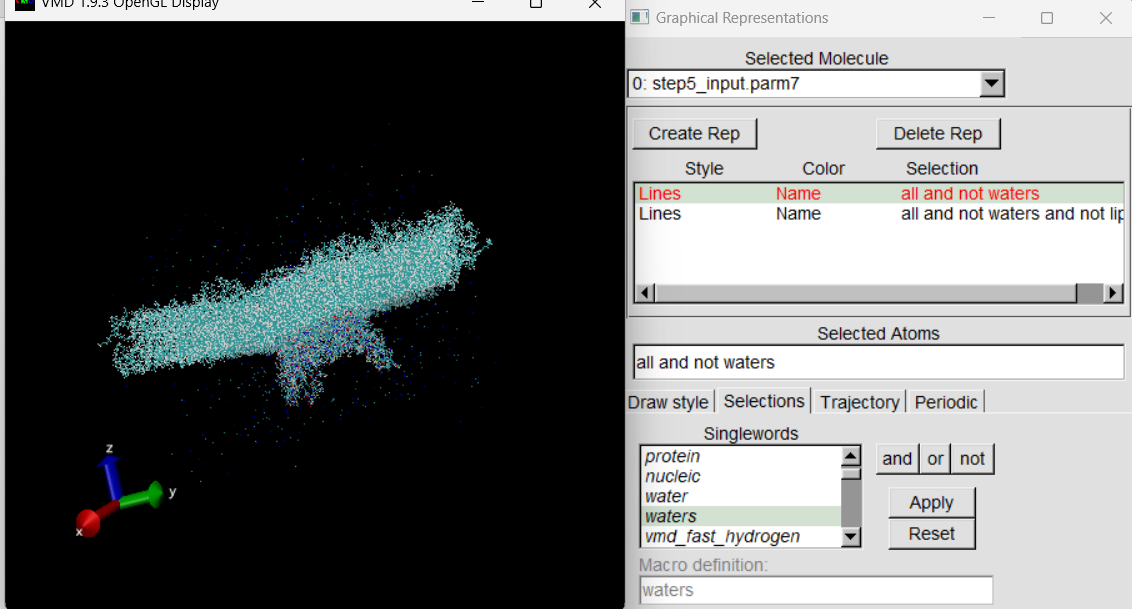
\includegraphics[width = 0.5\textwidth]{figs/lipid-rep.png}
\end{figure}

\newpage

Ahora repetimos lo mismo con el documento complex-vilazodone-p2x7.top y seleccionamos AMBER7 Parm como tipo. Cargamos y seleccionamos el short con la caja de agua. En representación, ponemos all with not waters. 

\begin{figure}[h]
\centering
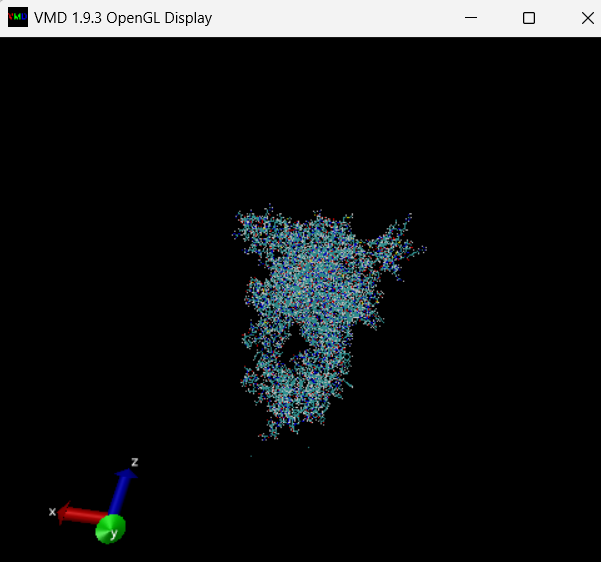
\includegraphics[width = 0.4\textwidth]{figs/protein-dynamics.png}
\end{figure}

Ponemos crear una representación con all and not waters and not protein para ver el ligando y cómo se mueve con las distintas conformaciones. 

En la pestaña principal, podemos dar click derecho y guardar las coordenadas. Se genera un documento pdb en el que está la tabla.

\begin{figure}[h]
\centering
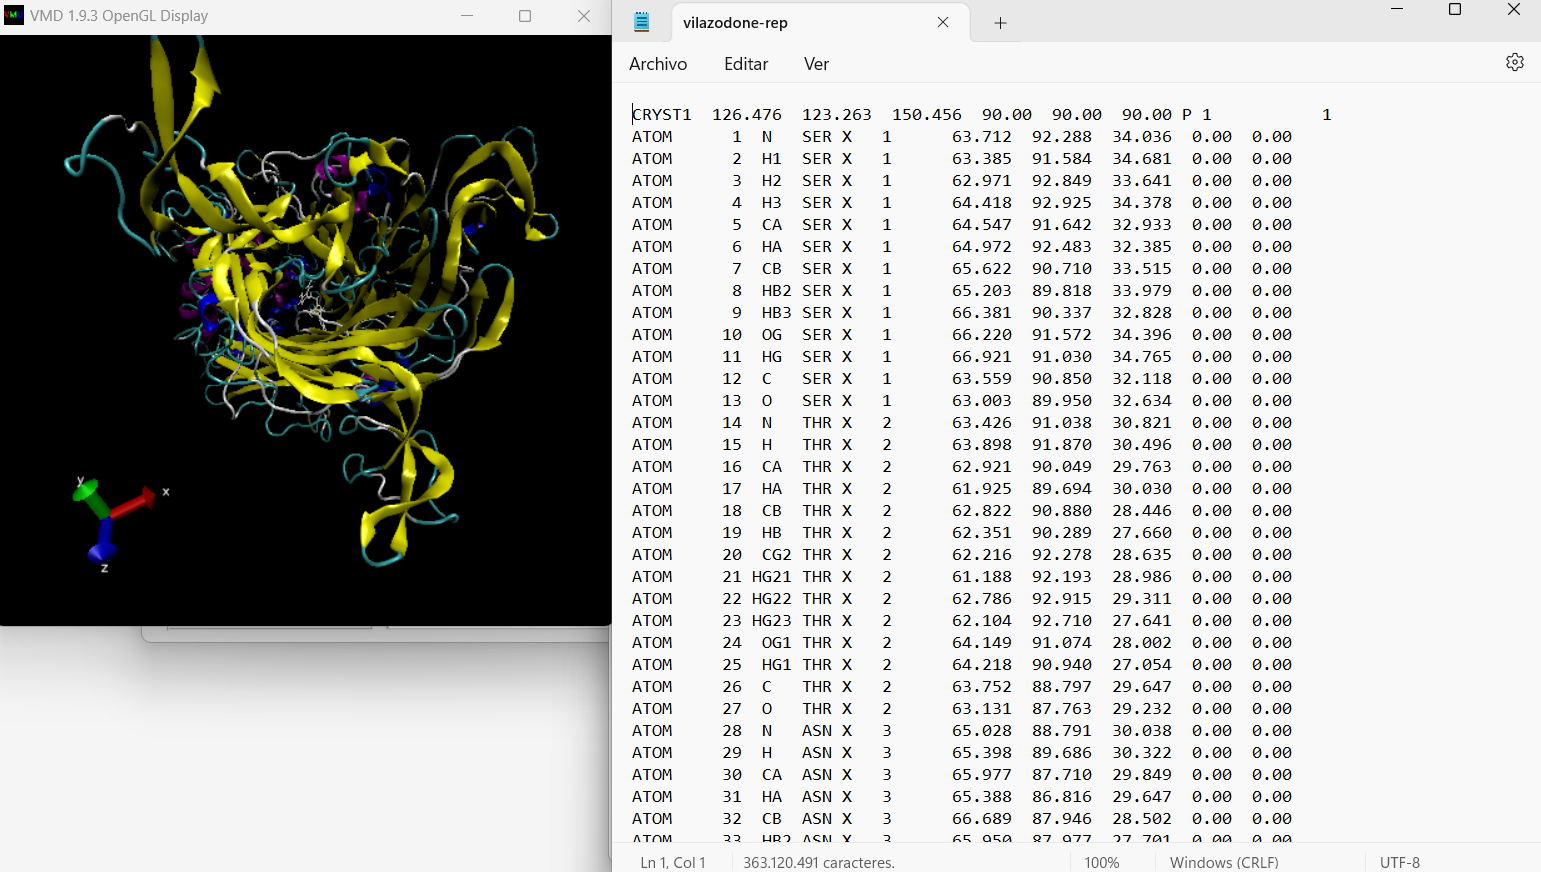
\includegraphics[width = 0.7\textwidth]{figs/md-tabla.png}
\end{figure}

Ahora abrimos Discovery Studio y abrimos el documento complex\_orai1\_telmisartan. Este contiene la proteína. Abrimos el documento de complex\_telmisartan y tenemos el ligando. Pulsamos con click derecho en el ligando y seleccionamos Custom Carbon atoms only y ponemos un color azul. De la misma forma lo copiamos y pegamos con la proteína. Ahora debemos seleccionar solo el ligando e ir a Receptor-Ligand Interaction > Ligand Interactions. En Interaction Options desseleccionamos Show Intramolecular interactions en la parte de abajo. Con click derecho se pueden añadir etiquetas, y se puede mostrar un diagrama 2D de las interacciones y sus tipos.

\begin{figure}[h]
\centering
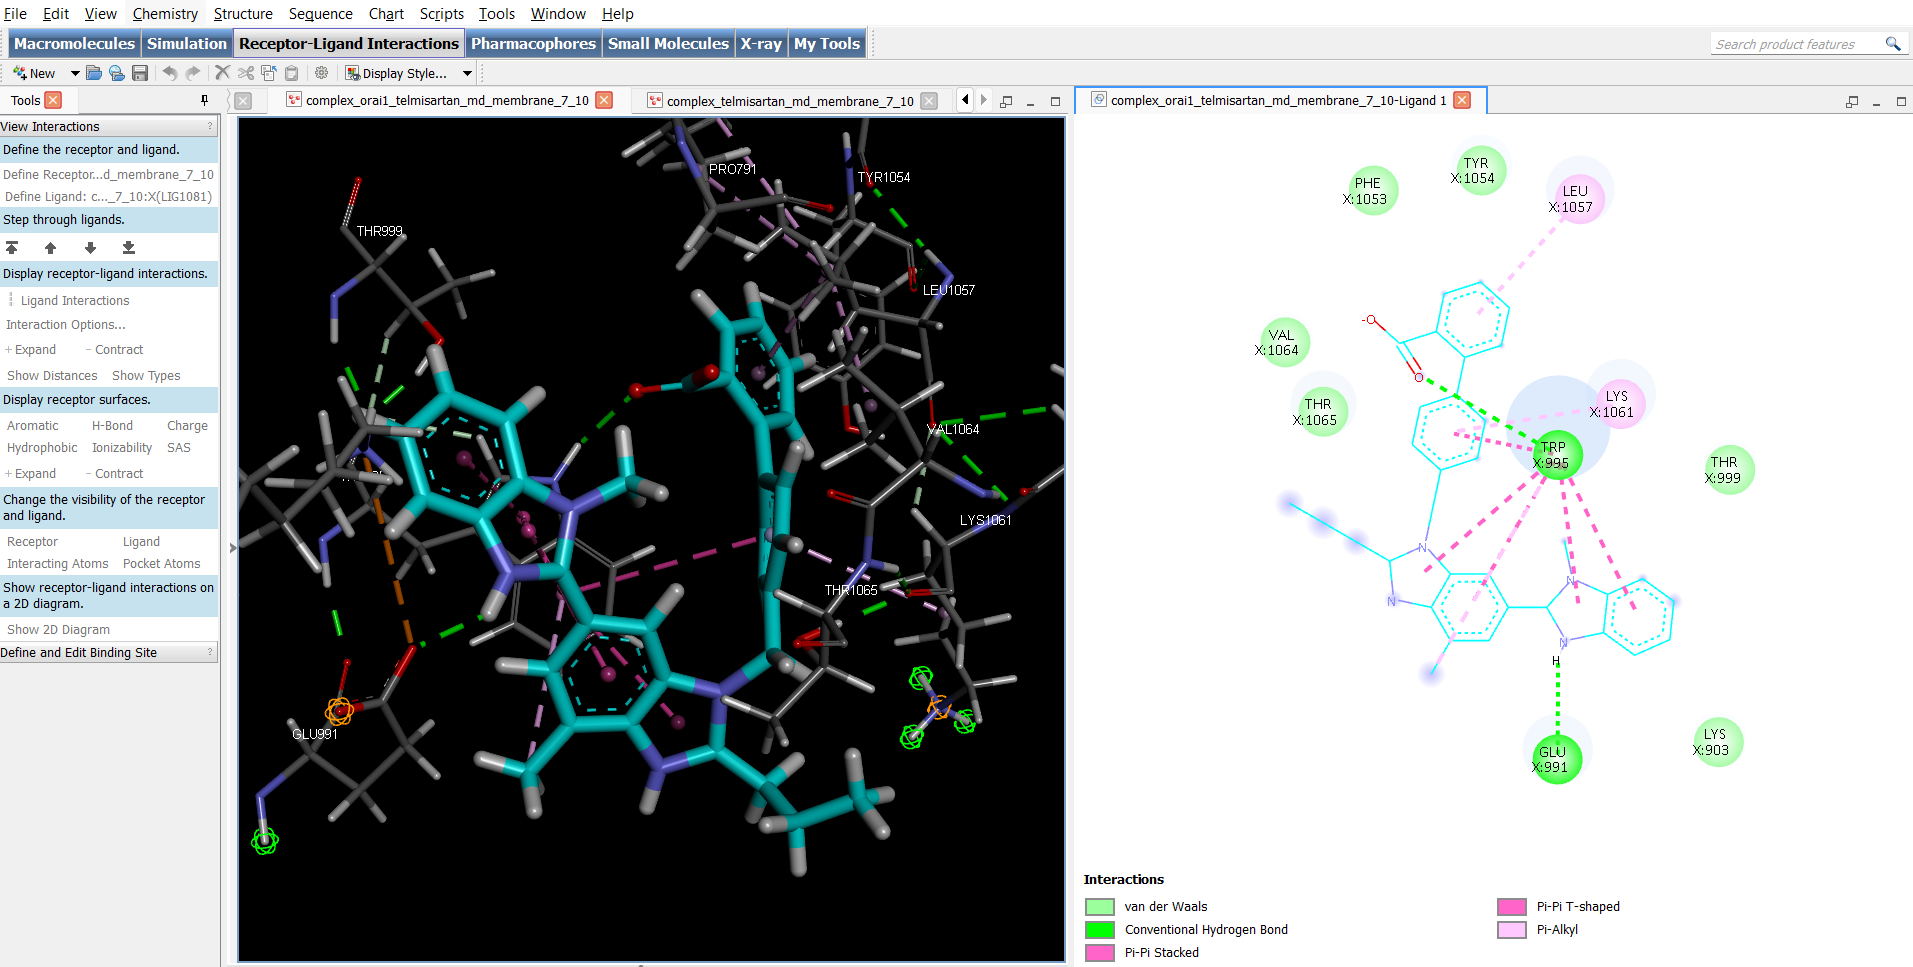
\includegraphics[width = 0.7\textwidth]{figs/2d-diagram-docking.png}
\end{figure}

Volvemos a abrir el fichero con la proteína sola. En la parte izquierda nos vamos a Define and Edit Binding Site y From Receptor Cavities. Al lado del panel hay una flechita que podemos expandir. Ahí sale una lista con los posibles sitios de unión. 

\begin{figure}[h]
\centering
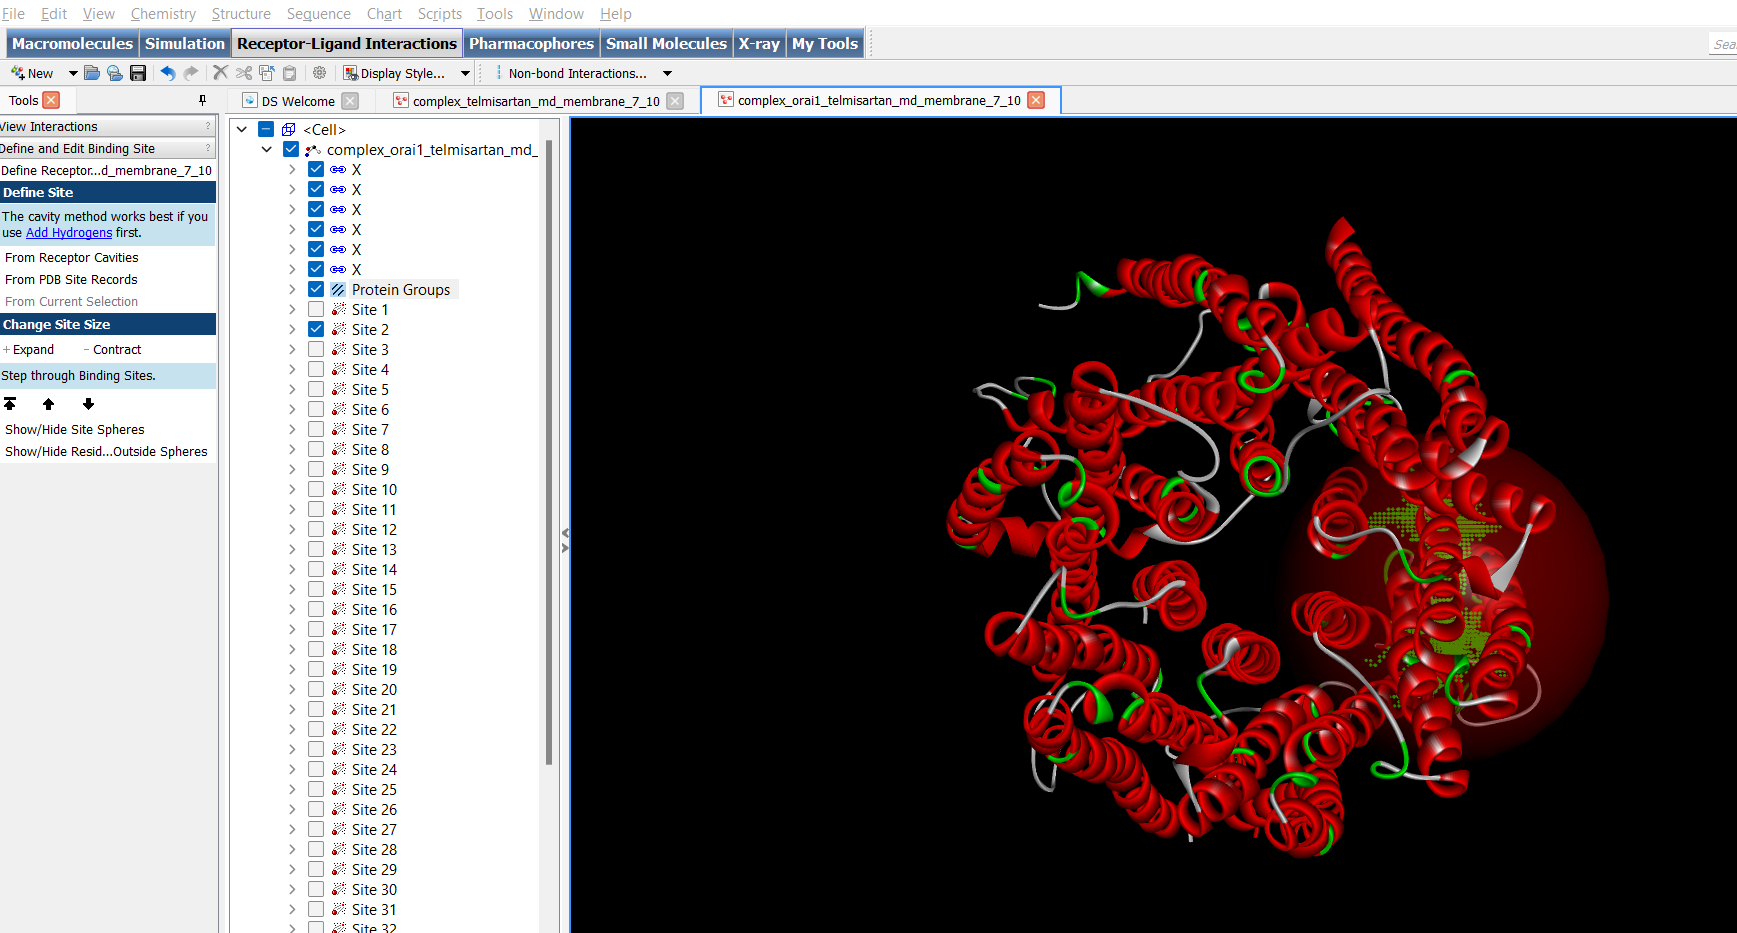
\includegraphics[width = 0.7\textwidth]{figs/binding-sites.png}
\end{figure}

Copiamos el fichero docking.pdbqt para duplicarlo. Lo llamamos lig1 para quedarnos solo con el primer modelo. Aprovechamos también para limpiar el fichero. Eliminamos todos los modelos que no sean el 1, eliminamos la cabecera, eliminamos todos los ROOT, BRANCH, ENDBRANCH y demás, y al final también eliminamos todo. Nos debemos quedar sólo con HETATM, y tras la última fila añadimos TER y END. Discovery Studio no reconoce los ficheros PDBQT de Docking, por lo que podemos abrirlos en PyMOL, ir a Export Molecule y exportarlo a PDB.